%\documentclass{article}
%\usepackage{graphicx,subfigure}
%\begin{document}

\begin{figure}[!h]
  \centering
   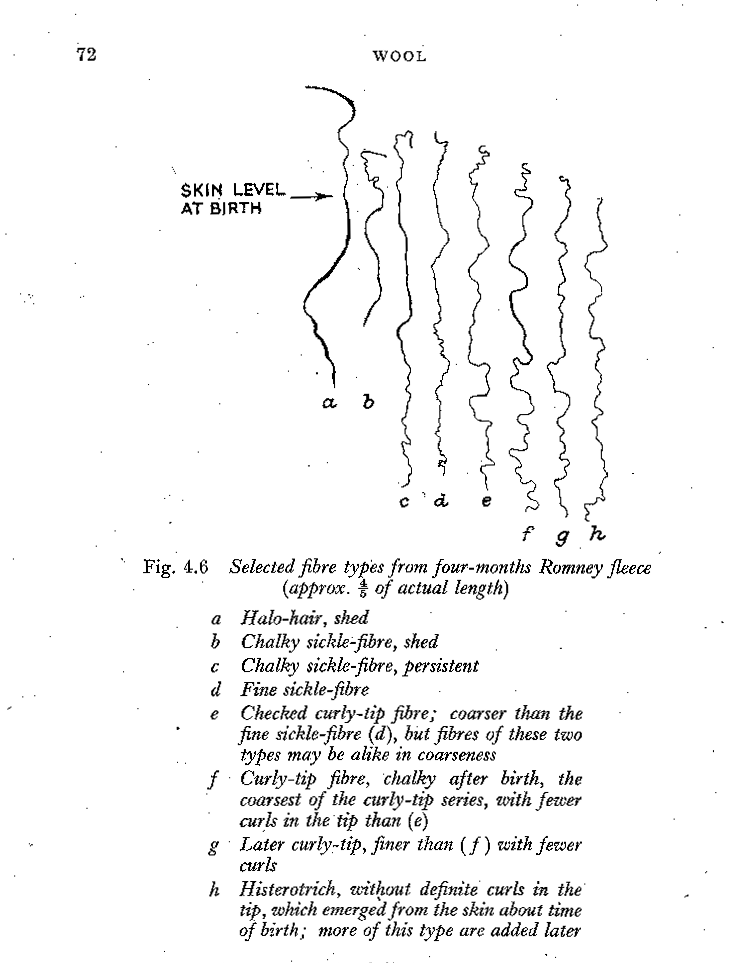
\includegraphics[width=1.0\textwidth]{onions2.png}
  \caption{Figure from Onions(1962)~\cite{onio:62} showing fibre types from a Romney lamb with the  fibres aligned according to the position of the skin level at birth}
  \label{fig:onions}
\end{figure}

%\end{document}

